\documentclass[11pt,a4paper,DIV=14,headinclude=false,footinclude=false]{scrartcl}
\usepackage[utf8]{inputenc}
%!TeX spellcheck = en_GB
\usepackage[english]{babel}
\usepackage[T1]{fontenc}
\usepackage{lmodern}

\usepackage{enumitem} % Extended enumerate: label= ...
\usepackage{listings} % Code formatting
% Math
%\usepackage{amsmath}
\usepackage{mathtools} % amsmath extension
\usepackage{amsfonts} % Math fonts
\usepackage{amssymb}
%\usepackage{amsthm} % Theorems, like proof
%\usepackage{stmaryrd} % More symbols, like \lightning, rrbracket, ...
% Tables
\usepackage{array} % Extended options for array and tabular
\usepackage{booktabs} % Rules for tables
%\usepackage{tabu} % Extended table environment
% Graphics and floats
\usepackage{graphicx}
%\usepackage{placeins} % \FloatBarrier
%\usepackage{float} % [H] for floats
% Refs
\usepackage[bookmarks=true,bookmarksnumbered=true,colorlinks=false,linkbordercolor={0 0 0},pdfborder={0 0 0}]{hyperref}
%\usepackage[all]{hypcap} % Link to top of figure and table
\usepackage{caption}
\usepackage{lastpage}

% Style
\setkomafont{captionlabel}{\bfseries}
\setcounter{secnumdepth}{-1} % Disables chapter and section numbering
%% Margins
%%\usepackage[top=2.5cm,head=2.5cm,headsep=0.5cm,inner=2cm,outer=2cm,bottom=2.5cm,footskip=1cm]{geometry}
%% Header and footer
\usepackage{scrlayer-scrpage}
\clearpairofpagestyles
\setkomafont{pageheadfoot}{\normalfont\sffamily}
%\pagestyle{scrheadings}
%%\setheadsepline{}[\ifthispageodd{}{\setheadsepline{0pt}}] % No headsepline for even pages
%%========================%
%\lohead{\small\begin{tabular}{@{}l@{ }l}
%    Ralph Lesch
%\end{tabular}
%}
%\cohead{\bfseries Deep Learning Lab WS2018 -- Exercise 3}
%\rohead{2018-12-04}
%%
\cfoot[\pagemark/\pageref{LastPage}]{\pagemark/\pageref{LastPage}} % Site number

\begin{document}
\title{Deep Learning Lab WS2018\\Exercise 3}
\author{Ralph Lesch}
\maketitle

\noindent The topic of this exercise is semantic segmentation. We implement several decoder modules for Fully Convolutional Networks (FCNs) in 4 configurations:
\begin{enumerate}
\item a simple single stage decoder module, upsampling the encoder results via transposed convolution 16x to its original spatial resolution.
\item multi-stage decoder with 2x upsamling and a skip connection to refine the results.
\item 2x refinement with 2x upsamling.
\item 3x ref., also with 2x upsampling each.
\end{enumerate}
\section{Results}
Below you can see the maximum Intersection Over Union (IoU) for each configuration (\autoref{tab:maxIoU}) and their plots (\autoref{fig:all}, \ref{fig:single}). The difference between a single stage decoder (config 1) and the multi-stage decoders (config 2-4) is clearly visible. With three refinements / skip connections (config 4) the maximum IoU is 10x higher than without (config 1).

\begin{minipage}{.35\textwidth} \centering
    \captionsetup{type=table,justification=raggedright}
    \begin{tabular}{ccc}\toprule
        config & max(IoU) & epoch \\ \midrule
        1 & 0.03592 & 32\,000\\
        2 & 0.07798 & 36\,000\\
        3 & 0.22098 & 31\,000\\
        4 & 0.38193 & 40\,000\\ \bottomrule
    \end{tabular}
    \caption{Intersection ver Union (IoU)}\label{tab:maxIoU}
\end{minipage}\hfill
\begin{minipage}{.65\textwidth} \centering
    \captionsetup{type=figure}
    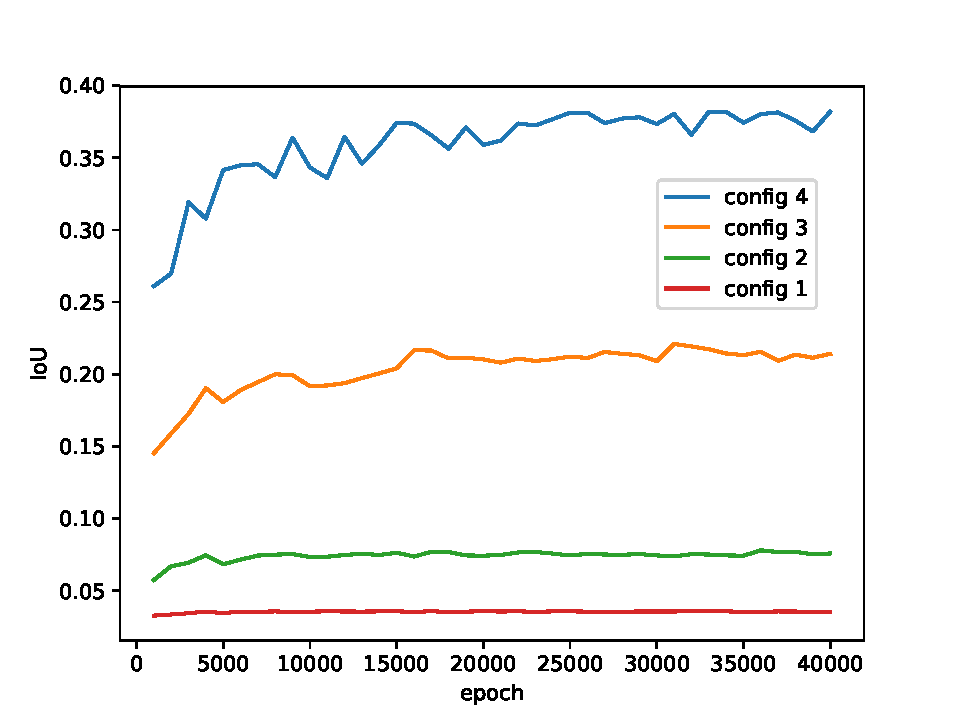
\includegraphics[width=\linewidth,keepaspectratio,clip,trim=0 0 30px 20px]{plots/configs.pdf}
    \caption{IoU vs epoch plot of all configurations}
    \label{fig:all}
\end{minipage}

\noindent After a high increase of IoU at the first 5-10 thousand epochs (longer with more refinements), the curves saturate, with only a small increase in IoU. With overall higher and longer increasing IoU (until saturation), config 4, with the most refinements is clearly the best decoder here.

\begin{figure}[h]\centering
    \begin{minipage}{.5\textwidth} \centering
        config 1
        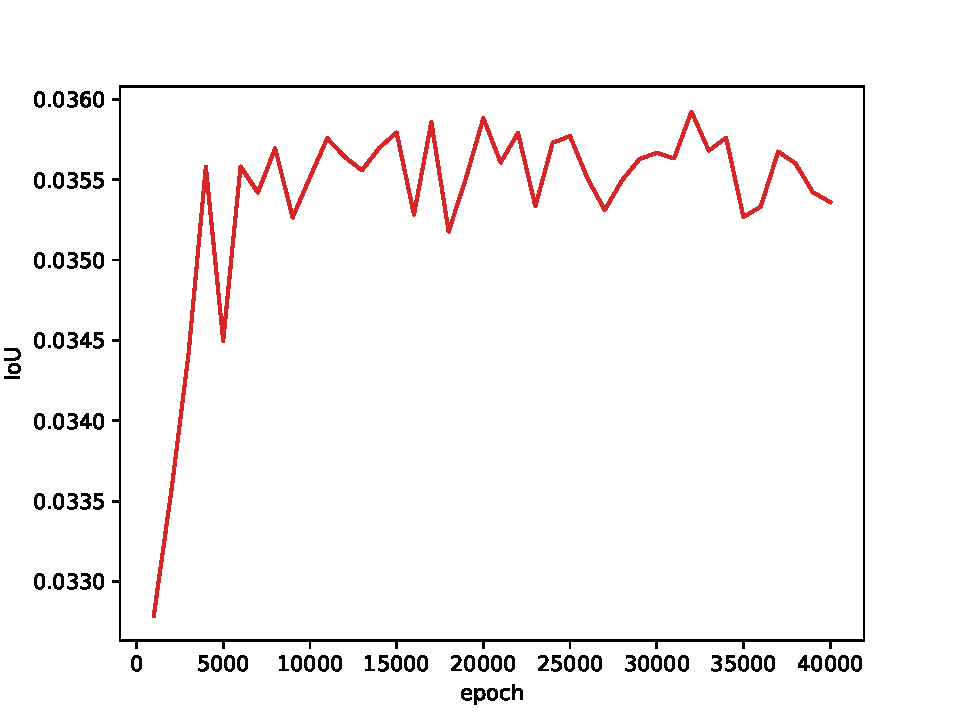
\includegraphics[width=\linewidth,keepaspectratio,clip,trim=0 0 30px 30px]{plots/config1.pdf}
%        \caption{config 1}
    \end{minipage}\hfill
    \begin{minipage}{.5\textwidth}\centering
        config 2
        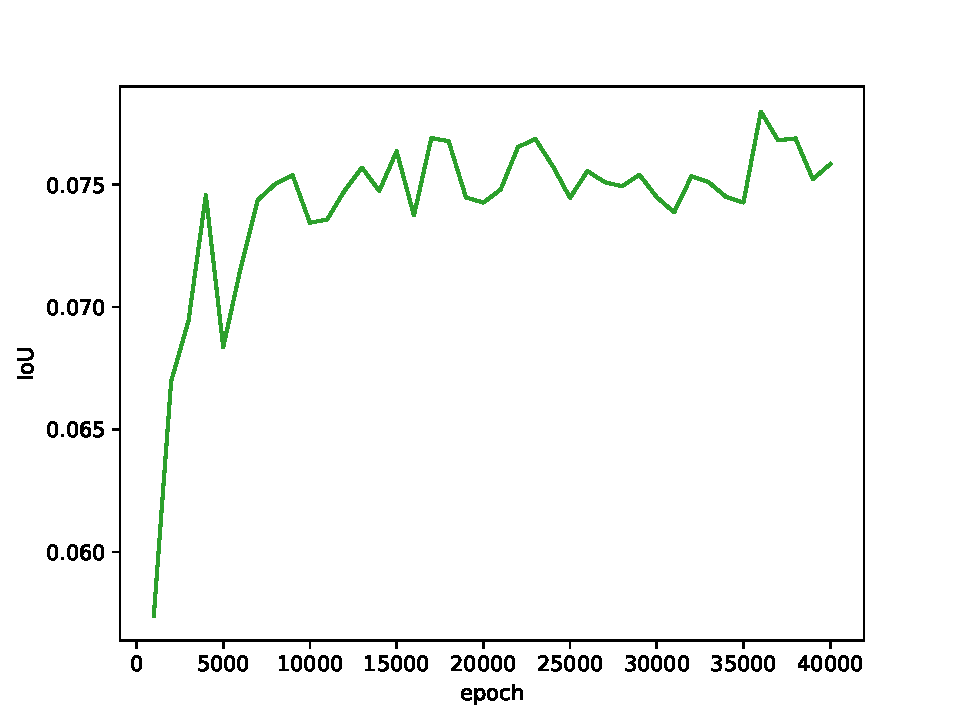
\includegraphics[width=\linewidth,keepaspectratio,clip,trim=0 0 30px 30px]{plots/config2.pdf}
%        \caption{config 2}
     \end{minipage}\\[\baselineskip]
%\end{figure}
%\begin{figure}[hbt]\centering
    \begin{minipage}{.5\textwidth} \centering
        config 3
        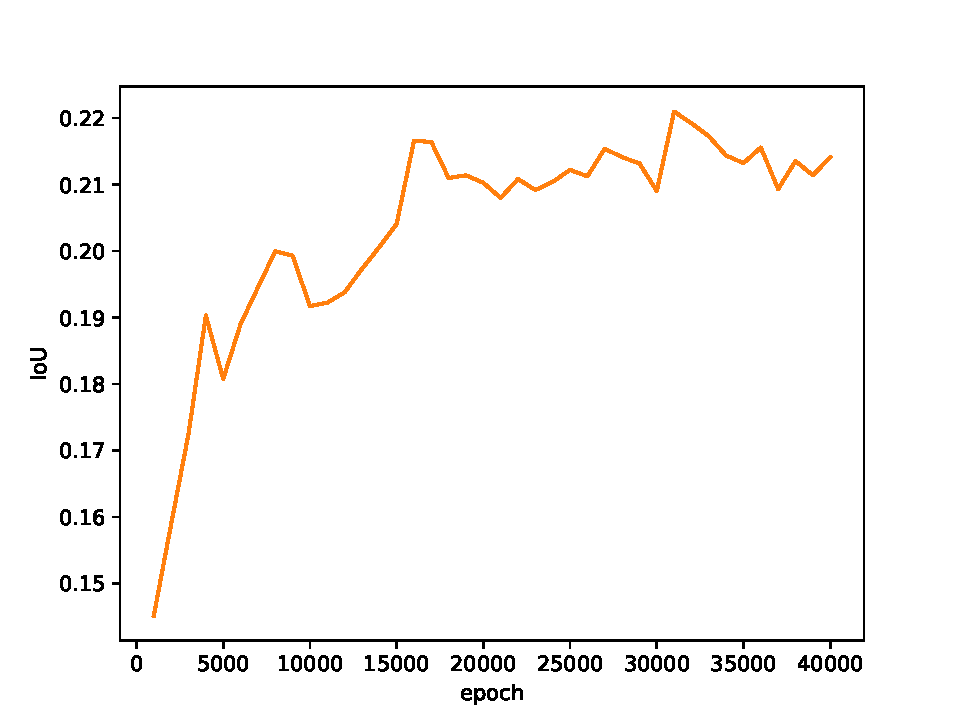
\includegraphics[width=\linewidth,keepaspectratio,clip,trim=0 0 30px 30px]{plots/config3.pdf}
%        \caption{config 3}
    \end{minipage}\hfill
    \begin{minipage}{.5\textwidth}\centering
        config 4
        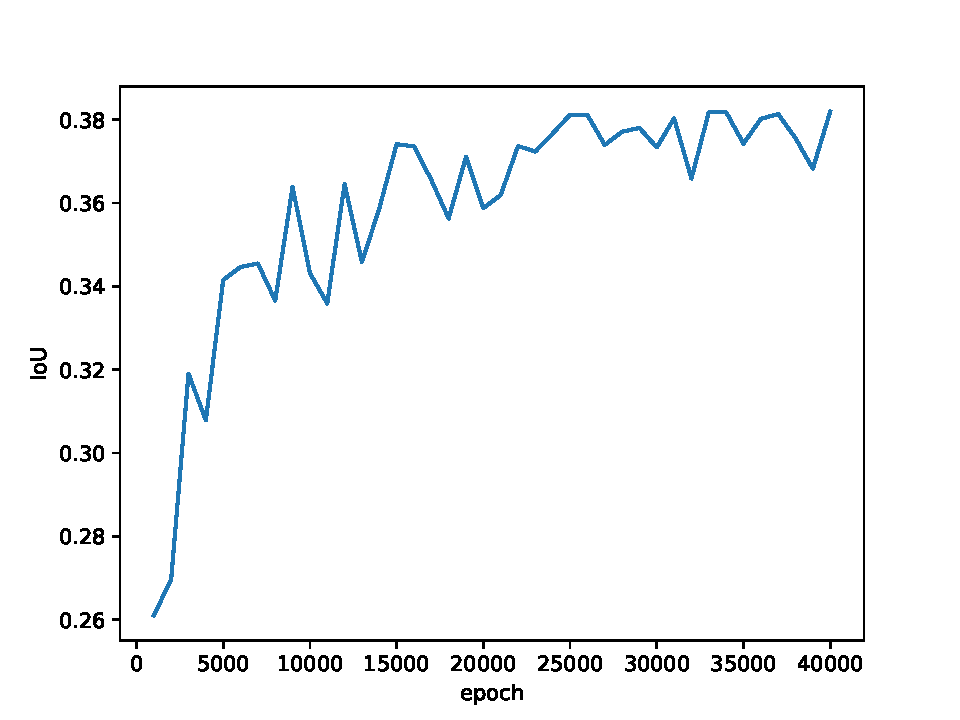
\includegraphics[width=\linewidth,keepaspectratio,clip,trim=0 0 30px 30px]{plots/config4.pdf}
%        \caption{config 4}
     \end{minipage}
     \caption{plot for each configuration}\label{fig:single}
\end{figure}

\end{document}
